\section{Introduction}\label{introduction}

\begin{frame}{Basic Analyses}

\center
\textbf{Basic Analyses}: The analyses taught in the first stats course
\vspace{12pt}

\columnsbegin

\begin{column}{0.48\textwidth}
   These include:
   \begin{enumerate}
   \item T-tests
   \item ANOVA
   \item Linear Regression
   \end{enumerate}
   These allow us to assess relationships like that in the figure.
\end{column}\begin{column}{0.48\textwidth}
    \begin{center}
     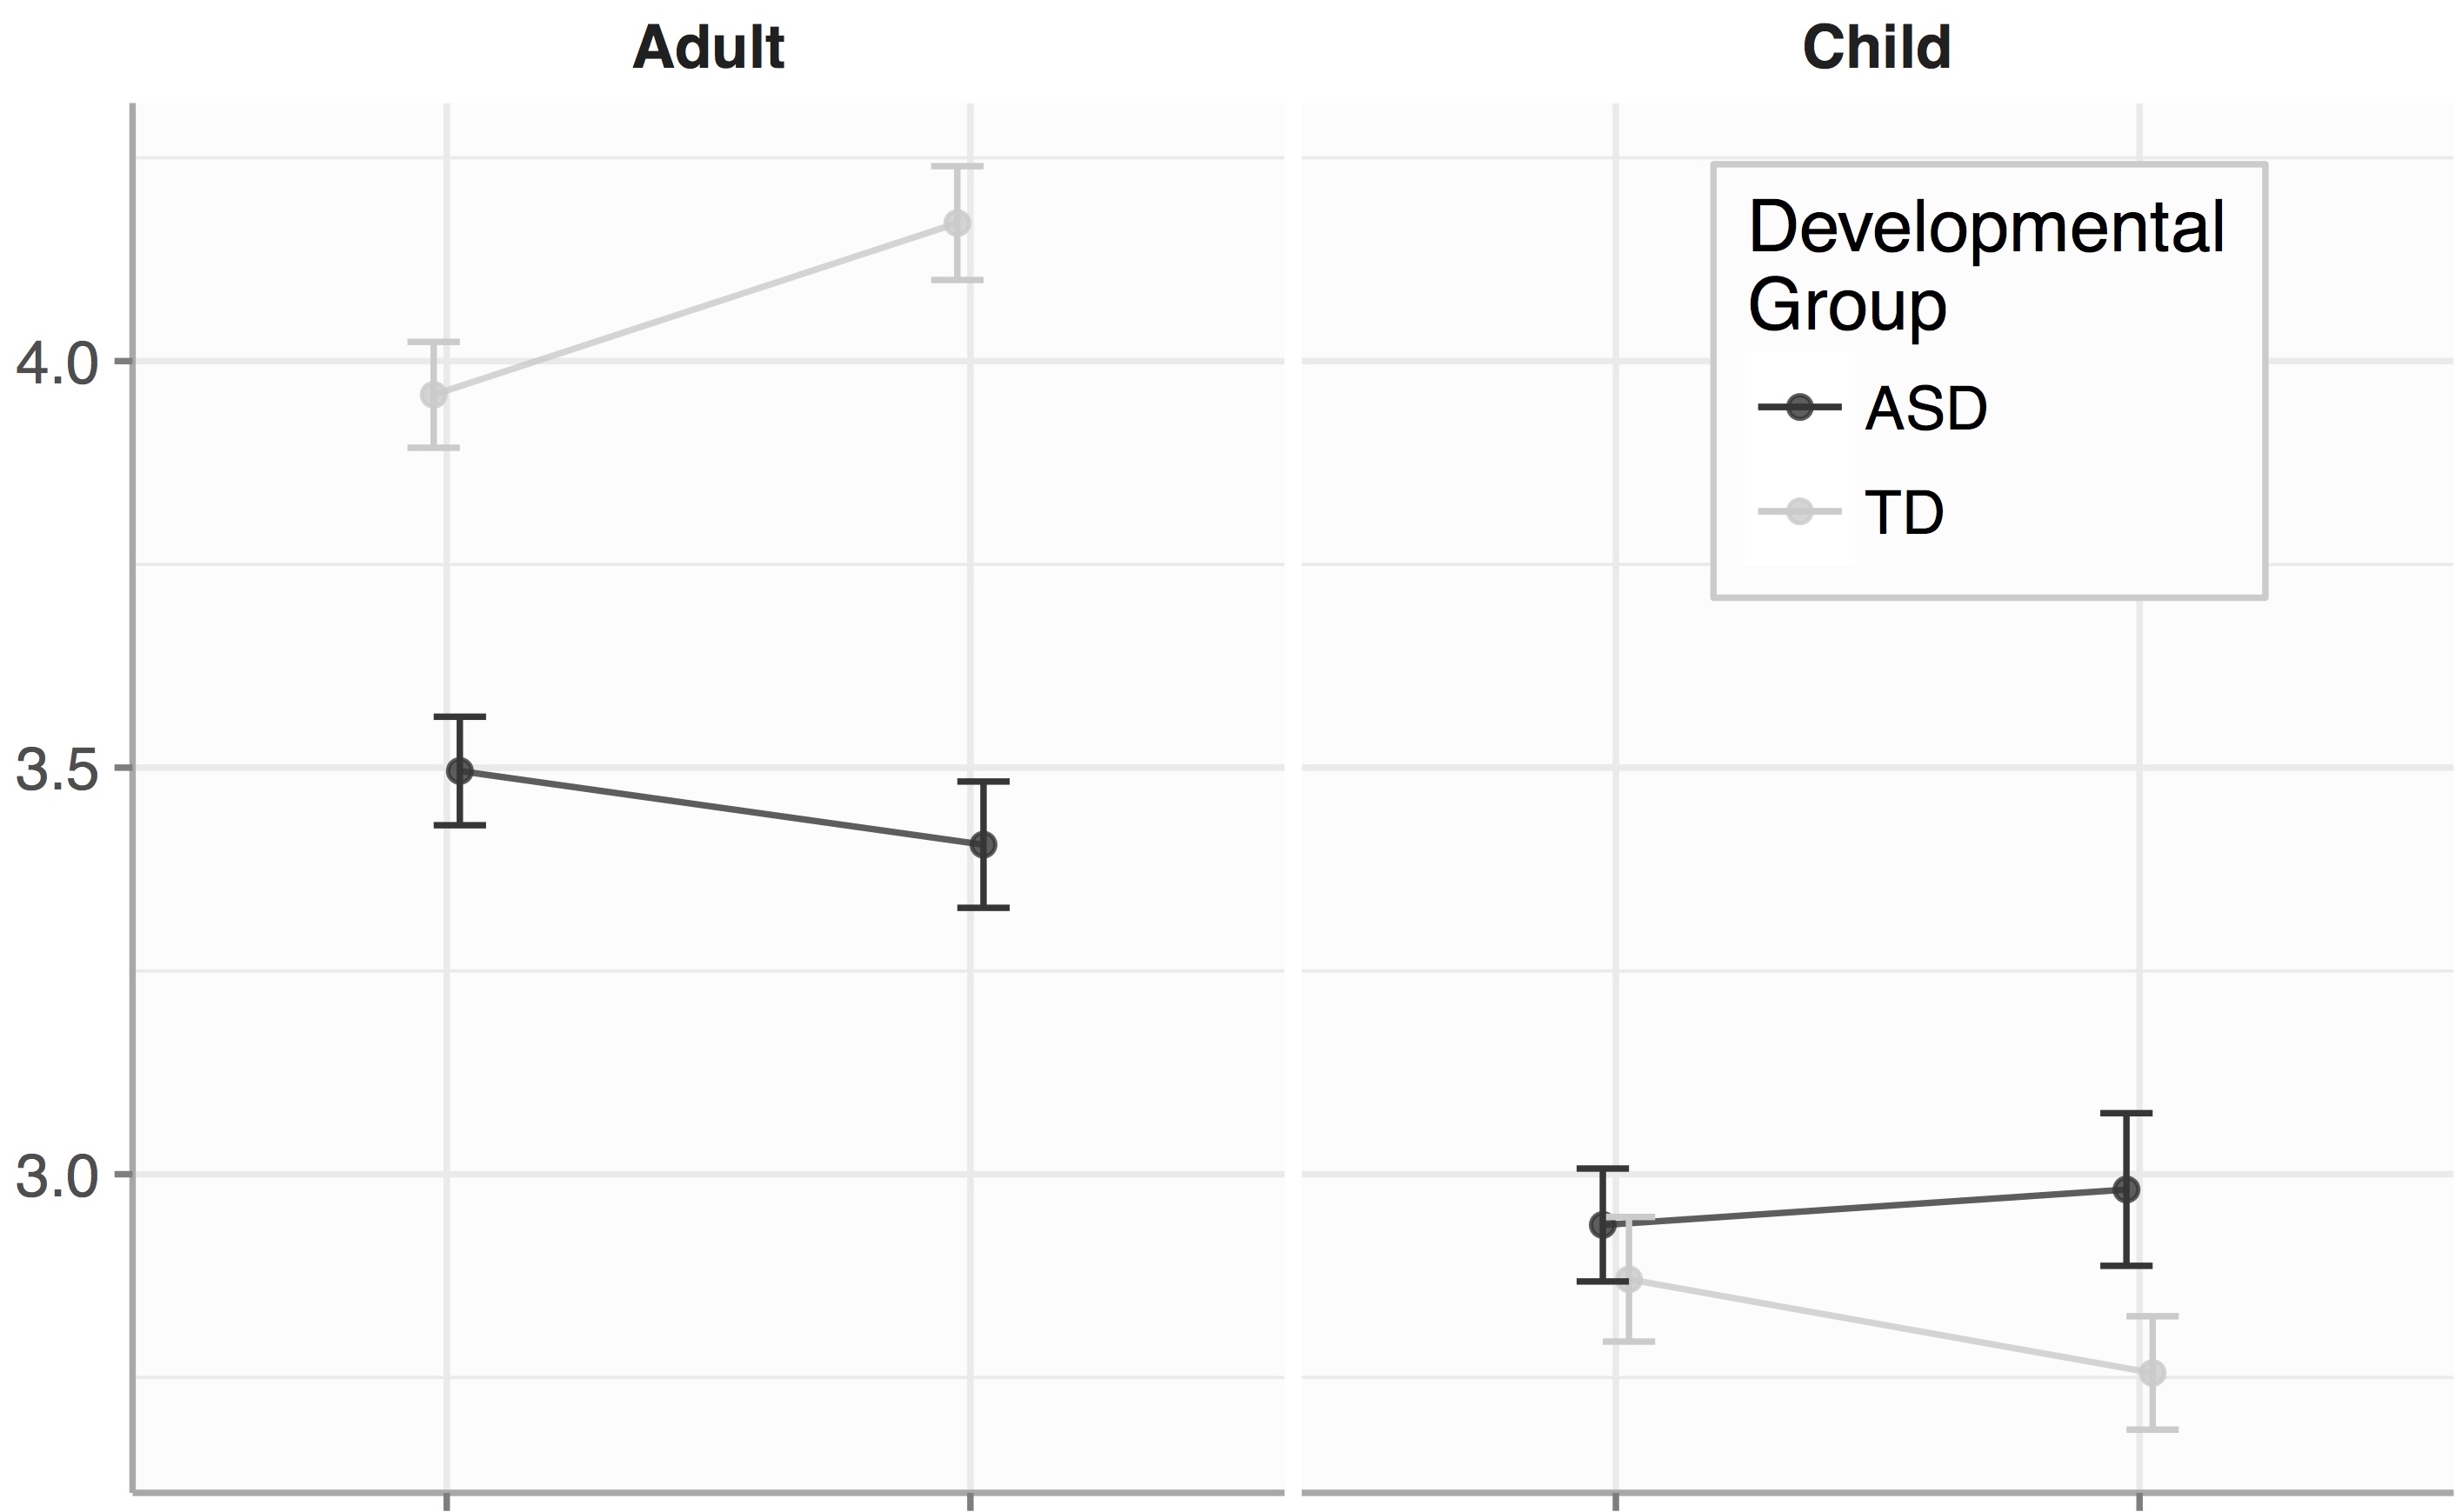
\includegraphics[width=\textwidth]{Figures/FigureInteraction.jpg}
     \end{center}
\end{column}

\columnsend

\vspace{12pt} Maybe surprising:\textbackslash{} These all are doing
essentially the same thing!

First, \textbf{T-TESTS!}

\end{frame}

\section{T-tests}\label{t-tests}

\begin{frame}{Three Types}

\Huge

\begin{enumerate}
\item Simple
\item Independent Samples
\item Paired Samples
\end{enumerate}

\end{frame}

\begin{frame}[fragile]{Three Types}

\Large
Each will be demonstrated using:

\normalsize

\begin{Shaded}
\begin{Highlighting}[]
\NormalTok{df <-}\StringTok{ }\KeywordTok{data.frame}\NormalTok{(}\StringTok{"A"}\NormalTok{=}\KeywordTok{sample}\NormalTok{(}\KeywordTok{c}\NormalTok{(}\DecValTok{0}\NormalTok{,}\DecValTok{1}\NormalTok{), }\DecValTok{100}\NormalTok{, }\DataTypeTok{replace =} \OtherTok{TRUE}\NormalTok{),}
                 \StringTok{"B"}\NormalTok{=}\KeywordTok{rnorm}\NormalTok{(}\DecValTok{100}\NormalTok{),}
                 \StringTok{"C"}\NormalTok{=}\KeywordTok{rnorm}\NormalTok{(}\DecValTok{100}\NormalTok{))}
\NormalTok{df}
\end{Highlighting}
\end{Shaded}

\begin{verbatim}
    A            B            C
1   0 -0.888158433  0.294452230
2   1  0.384032654 -2.022480886
3   0 -0.978200548  0.363196635
4   0  0.597665769  0.306536631
5   0  0.849400438 -0.444227641
6   0 -0.890268979 -1.254064551
7   0 -0.854688613  0.938866598
8   0 -0.148777057 -2.283803888
9   0  1.046238407 -0.149862421
10  1  0.319170505 -0.607516590
11  0 -0.944016300  0.146733367
12  1 -1.137319922 -0.844196714
13  1 -0.289090610  1.092515855
14  0  1.560632013  0.651127439
15  1 -0.263143478 -0.407457050
16  0 -0.459680757  1.704288064
17  0  0.323325735  0.626672231
18  0  0.213562691  0.662002688
19  0 -1.453132131  1.814689637
20  0  0.259589469 -0.623349969
21  1 -2.178687938 -1.479540650
22  0 -0.988769699  1.284586615
23  1 -0.538773530 -0.120741596
24  1  0.890577789 -1.814290296
25  0 -0.373879908 -1.092930391
26  1 -0.009260305  0.003694269
27  0 -0.345341921 -1.571554185
28  1  1.083044516  1.072004889
29  1 -1.117759587 -2.123290725
30  0 -0.262098239  0.479728656
31  0  1.470558960 -0.837701203
32  0  1.639100045 -0.894385779
33  0 -0.026585310  0.041571565
34  0  1.838690589  1.221191733
35  0 -1.133964902 -1.465824944
36  1  1.452969579 -0.101763836
37  1 -0.372847527 -0.461312871
38  0  1.700370902  0.927889552
39  0 -0.535479976  1.056323868
40  0 -1.131767510 -0.672638075
41  1  1.395932675 -0.105853008
42  0  1.765105281  1.378744025
43  0  0.443446267  0.588502968
44  1  1.303825950 -0.523592469
45  0  0.870577900 -1.223672782
46  1 -1.146946332 -0.426095931
47  0 -0.590869948 -1.930208534
48  1 -1.420271789 -1.831663448
49  0  0.677192508 -1.149003074
50  1 -0.999263317  0.639276554
51  0  0.832485361 -0.142725862
52  0 -1.635758469 -0.485126605
53  0  1.109253880  0.254396299
54  1  1.063150237  1.245045134
55  0 -0.159479173  0.306450913
56  1  0.277330950 -0.504714998
57  1 -0.867404778 -0.435754652
58  1 -0.170515002  0.019615965
59  1  0.106589334 -0.427008864
60  1  1.894259526 -1.270702255
61  0 -0.942124829 -0.380465236
62  1 -0.039598443 -0.659031841
63  1  1.414352903  0.252853923
64  0 -0.386421046  0.150728792
65  0  0.734608554 -0.937463779
66  0  1.990269169  0.032838408
67  1  0.601033749  0.861801349
68  1 -1.833923459  0.054668982
69  0  0.934053588  1.368477005
70  0  0.876636108  1.177152155
71  0 -0.036131656 -1.498249323
72  0  1.002657856  0.928034423
73  1 -0.640870937 -0.950708502
74  0  2.531171125  0.508684580
75  1 -1.370268170 -1.213704565
76  0 -0.488117300 -0.788916854
77  0  0.051069136  0.673629670
78  1 -1.617188811  1.840895857
79  0 -0.006527606  0.144377906
80  1  0.437204284  0.061432246
81  0  0.034534899  0.643956234
82  0  0.336423631 -0.635485044
83  0  0.157964627 -0.368213528
84  1 -0.899991972  2.209238040
85  1 -0.278430139 -2.652066702
86  1 -1.360811557 -0.346753431
87  0 -2.668015333 -0.155135945
88  0  1.527740457  0.738530913
89  1 -0.404112818 -0.798185691
90  1 -0.640109871 -1.205627072
91  0  0.276161149 -0.246470241
92  0 -1.131874210 -1.584447113
93  1  0.653973257  0.035954617
94  1  1.106458336 -0.363543152
95  1  0.973976451 -1.978319501
96  0 -0.156593739 -0.419389703
97  0 -1.240219334 -1.956838650
98  0 -1.854956798  1.427759943
99  1  1.638895028 -1.372163472
100 1  0.789631195 -0.874194829
\end{verbatim}

\end{frame}

\begin{frame}[fragile]{Simple}

\center
Comparing a mean of a variable with \(\mu\).

\begin{Shaded}
\begin{Highlighting}[]
\KeywordTok{t.test}\NormalTok{(df}\OperatorTok{$}\NormalTok{B, }\DataTypeTok{mu =} \DecValTok{0}\NormalTok{)}
\end{Highlighting}
\end{Shaded}

\begin{verbatim}

    One Sample t-test

data:  df$B
t = 0.29332, df = 99, p-value = 0.7699
alternative hypothesis: true mean is not equal to 0
95 percent confidence interval:
 -0.1803399  0.2429081
sample estimates:
 mean of x 
0.03128405 
\end{verbatim}

\end{frame}

\begin{frame}[fragile]{Independent Samples}

\center
Comparing the means of two groups (\texttt{dfA} is the grouping
variable).

\begin{Shaded}
\begin{Highlighting}[]
\KeywordTok{t.test}\NormalTok{(df}\OperatorTok{$}\NormalTok{B }\OperatorTok{~}\StringTok{ }\NormalTok{df}\OperatorTok{$}\NormalTok{A)}
\end{Highlighting}
\end{Shaded}

\begin{verbatim}

    Welch Two Sample t-test

data:  df$B by df$A
t = 0.59367, df = 89.632, p-value = 0.5542
alternative hypothesis: true difference in means is not equal to 0
95 percent confidence interval:
 -0.3009458  0.5574410
sample estimates:
mean in group 0 mean in group 1 
     0.08514805     -0.04309956 
\end{verbatim}

\end{frame}

\begin{frame}[fragile]{Paired Samples}

\center
Comparing repeated measures (e.g., Pretest vs.~Posttest).

\begin{Shaded}
\begin{Highlighting}[]
\KeywordTok{t.test}\NormalTok{(df}\OperatorTok{$}\NormalTok{B, df}\OperatorTok{$}\NormalTok{C, }\DataTypeTok{paired =} \OtherTok{TRUE}\NormalTok{)}
\end{Highlighting}
\end{Shaded}

\begin{verbatim}

    Paired t-test

data:  df$B and df$C
t = 1.7086, df = 99, p-value = 0.09066
alternative hypothesis: true difference in means is not equal to 0
95 percent confidence interval:
 -0.03873655  0.51897089
sample estimates:
mean of the differences 
              0.2401172 
\end{verbatim}

\end{frame}

\begin{frame}[fragile]{Testing Assumptions of T-Tests}

T-tests require that the data be normally distributed with approximately
the same variance.

\begin{Shaded}
\begin{Highlighting}[]
\NormalTok{## Normality}
\KeywordTok{par}\NormalTok{(}\DataTypeTok{mfrow =} \KeywordTok{c}\NormalTok{(}\DecValTok{1}\NormalTok{,}\DecValTok{2}\NormalTok{))}
\KeywordTok{hist}\NormalTok{(df}\OperatorTok{$}\NormalTok{B)}
\KeywordTok{qqnorm}\NormalTok{(df}\OperatorTok{$}\NormalTok{B)}
\KeywordTok{abline}\NormalTok{(}\DataTypeTok{a=}\DecValTok{0}\NormalTok{, }\DataTypeTok{b=}\DecValTok{1}\NormalTok{)}
\end{Highlighting}
\end{Shaded}

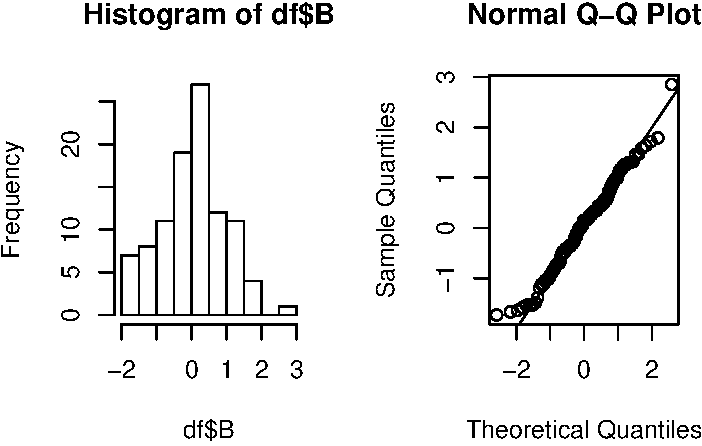
\includegraphics{04_BasicAnalyses_files/figure-beamer/unnamed-chunk-5-1.pdf}

\begin{Shaded}
\begin{Highlighting}[]
\NormalTok{## Variance}
\KeywordTok{var}\NormalTok{(df}\OperatorTok{$}\NormalTok{B)}
\end{Highlighting}
\end{Shaded}

\begin{verbatim}
[1] 1.1375
\end{verbatim}

\begin{Shaded}
\begin{Highlighting}[]
\KeywordTok{var}\NormalTok{(df}\OperatorTok{$}\NormalTok{C)}
\end{Highlighting}
\end{Shaded}

\begin{verbatim}
[1] 1.077731
\end{verbatim}

\end{frame}

\section{ANOVA}\label{anova}

\begin{frame}[fragile]{Analysis of Variance}

The Analysis of Variance (ANOVA) is highly related to t-tests but can
handle 2+ groups.

\begin{enumerate}
\def\labelenumi{\arabic{enumi}.}
\tightlist
\item
  Provides the same p-value as t-tests
\item
  \(t^2\) = \(F\)
\end{enumerate}

For example:

\begin{Shaded}
\begin{Highlighting}[]
\NormalTok{fit_ano =}\StringTok{ }\KeywordTok{aov}\NormalTok{(df}\OperatorTok{$}\NormalTok{B }\OperatorTok{~}\StringTok{ }\NormalTok{df}\OperatorTok{$}\NormalTok{A)}
\KeywordTok{summary}\NormalTok{(fit_ano)}
\end{Highlighting}
\end{Shaded}

\begin{verbatim}
            Df Sum Sq Mean Sq F value Pr(>F)
df$A         1    0.4  0.4007    0.35  0.556
Residuals   98  112.2  1.1450               
\end{verbatim}

\begin{Shaded}
\begin{Highlighting}[]
\KeywordTok{t.test}\NormalTok{(df}\OperatorTok{$}\NormalTok{B }\OperatorTok{~}\StringTok{ }\NormalTok{df}\OperatorTok{$}\NormalTok{A)}\OperatorTok{$}\NormalTok{p.value}
\end{Highlighting}
\end{Shaded}

\begin{verbatim}
[1] 0.5542261
\end{verbatim}

\end{frame}

\begin{frame}[fragile]{Analysis of Variance}

\begin{Shaded}
\begin{Highlighting}[]
\NormalTok{fit_ano =}\StringTok{ }\KeywordTok{aov}\NormalTok{(df}\OperatorTok{$}\NormalTok{B }\OperatorTok{~}\StringTok{ }\NormalTok{df}\OperatorTok{$}\NormalTok{A)}
\KeywordTok{summary}\NormalTok{(fit_ano)}
\KeywordTok{t.test}\NormalTok{(df}\OperatorTok{$}\NormalTok{B }\OperatorTok{~}\StringTok{ }\NormalTok{df}\OperatorTok{$}\NormalTok{A)}\OperatorTok{$}\NormalTok{p.value}
\end{Highlighting}
\end{Shaded}

Notice in the code:

\begin{itemize}
\tightlist
\item
  We assigned the \texttt{aov()} the name \texttt{fit\_ano} (which we
  could have called anything)
\item
  We used the \texttt{summary()} function to see the F and p values.
\item
  We pulled the p-value right out of the \texttt{t.test()} function.
\end{itemize}

\end{frame}

\begin{frame}{Types}

\huge

\begin{enumerate}
\item One-Way
\item Two-Way (Factorial)
\item Repeated Measures
\item A combination of Factorial and Repeated Measures
\end{enumerate}

\end{frame}

\begin{frame}[fragile]{Types}

We will use the following data set for the examples:

\begin{Shaded}
\begin{Highlighting}[]
\KeywordTok{library}\NormalTok{(tidyverse)}
\NormalTok{df <-}\StringTok{ }\KeywordTok{data.frame}\NormalTok{(}\StringTok{"A"}\NormalTok{=}\KeywordTok{sample}\NormalTok{(}\KeywordTok{c}\NormalTok{(}\DecValTok{0}\NormalTok{,}\DecValTok{1}\NormalTok{), }\DecValTok{100}\NormalTok{, }\DataTypeTok{replace =} \OtherTok{TRUE}\NormalTok{) }\OperatorTok\StringTok{ }\NormalTok{factor,}
                 \StringTok{"B"}\NormalTok{=}\KeywordTok{rnorm}\NormalTok{(}\DecValTok{100}\NormalTok{),}
                 \StringTok{"C"}\NormalTok{=}\KeywordTok{rnorm}\NormalTok{(}\DecValTok{100}\NormalTok{),}
                 \StringTok{"D"}\NormalTok{=}\KeywordTok{sample}\NormalTok{(}\KeywordTok{c}\NormalTok{(}\DecValTok{1}\OperatorTok{:}\DecValTok{4}\NormalTok{), }\DecValTok{100}\NormalTok{, }\DataTypeTok{replace =} \OtherTok{TRUE}\NormalTok{) }\OperatorTok\StringTok{ }\NormalTok{factor)}
\NormalTok{df}
\end{Highlighting}
\end{Shaded}

\begin{verbatim}
    A            B            C D
1   1  0.393203143  0.166533149 3
2   1  0.325532077  0.121702597 4
3   0 -0.716154628  0.208602755 3
4   0 -0.544302202  0.033837841 2
5   0 -1.040692589 -0.353863739 1
6   1  1.086275696 -0.249269105 2
7   0 -0.304352002 -1.226131107 2
8   1 -0.825585271 -1.068904014 4
9   0 -1.015497075  0.104556660 1
10  0 -0.045372941  0.794159163 4
11  1  1.459118937 -0.701351642 1
12  0 -0.353239448 -1.065720834 1
13  1 -0.546563951  0.873137266 4
14  0  0.858764972  1.047552566 2
15  0 -0.225617056  1.033550228 4
16  0  0.776643544  2.009654267 1
17  0  2.325127275  0.487928162 3
18  1  2.181468801 -0.133559657 2
19  1 -0.204125729  1.128053702 2
20  1 -0.166418245  0.806367511 1
21  1  0.117421843 -0.001619959 4
22  1  0.337828786  1.602134850 2
23  1  1.565014407  1.709133634 4
24  0 -0.262640205  0.485869402 4
25  1 -0.474295772  0.203416797 3
26  0 -0.004114832 -0.914419246 3
27  1 -0.182468335  0.130403333 4
28  1  1.279935378 -0.407265520 1
29  1 -0.369196628 -0.265501724 2
30  0 -1.339146712 -0.358160223 1
31  1 -1.819692384 -0.784082559 1
32  1 -1.272439482 -1.261962710 2
33  1 -0.085557127  0.652885544 4
34  1  1.662796086  0.817999082 2
35  1  0.017213908  1.363547406 1
36  0 -0.774782299 -0.277780699 4
37  0 -2.236284667  1.440817537 2
38  0 -0.490292694 -0.959724306 1
39  1  1.842274482 -1.169215833 1
40  0 -1.249453216  0.350871407 4
41  1 -2.136188553  1.545710579 3
42  1  0.561723800 -0.628199838 3
43  0  1.362463219  0.516584504 2
44  0  0.224140485  0.972578891 4
45  1  1.077345766 -0.094076327 4
46  0 -0.323870524  0.212464834 1
47  0  0.063902606 -0.060875947 1
48  0 -1.167631193  0.872796576 1
49  1 -0.546295031 -0.057727111 2
50  0  0.977863988 -1.629076711 4
51  1 -0.026067726  0.647011030 3
52  1  1.137523673 -1.031798203 3
53  1 -0.016758817 -0.218012540 4
54  1 -0.664152117  1.250229407 2
55  0 -1.473866547 -0.741159284 2
56  0 -1.216320216 -0.911625629 2
57  1  1.812254148 -1.684767393 1
58  0 -1.016385169  1.454542836 2
59  0  0.490672303  2.091128186 1
60  1 -0.381182214  1.331982929 1
61  1 -1.546286679  0.343054559 3
62  1  0.510124614 -1.241272137 1
63  1  0.113442474  0.201262122 1
64  1 -0.288454877  0.372106831 3
65  0  0.394300961 -0.624749989 2
66  1 -2.013346172  0.250869421 3
67  0  0.064566105  0.455031643 2
68  0 -2.452278510 -0.742081982 4
69  1 -0.042535619  1.116168567 3
70  0  0.865088627 -0.165894497 4
71  1 -0.181501413 -0.572195930 1
72  0 -1.164839795 -0.586905808 3
73  1 -0.506622969 -1.015504836 1
74  1 -1.785191868 -0.833908472 4
75  0  0.203326958  0.585411148 1
76  1  1.344769111  0.531038516 1
77  0  0.959443696 -1.511273765 2
78  0  0.428772208 -0.176417308 2
79  1 -0.986421914 -0.596550075 3
80  1 -0.934105425  0.087091339 1
81  1 -0.607875208  0.859421921 2
82  0  0.289450571  0.150278879 2
83  0  0.410712034  0.916913962 4
84  1 -2.209388954 -2.143021662 4
85  1  0.914928560  0.492065379 3
86  1 -0.241317645  1.195378581 2
87  1 -0.359508062 -0.979073575 3
88  1 -0.538064784 -0.137859032 1
89  1  1.313021199  1.067661198 2
90  1 -0.384631424  0.890441779 3
91  0  0.478821594  0.039159001 4
92  0  0.572846276 -1.249903174 2
93  0 -1.816010588 -1.274787429 1
94  1 -0.145093229 -0.484864405 3
95  0  0.186880347  0.712270555 1
96  1  0.075494764 -0.535698319 4
97  1 -0.685747475 -0.095658067 4
98  1 -0.286583634 -1.150643075 4
99  1 -0.665652351  1.954924795 3
100 0 -0.551060832  0.574255887 3
\end{verbatim}

\end{frame}

\begin{frame}[fragile]{One-Way}

A One-Way ANOVA can be run using \texttt{aov()}.

\begin{Shaded}
\begin{Highlighting}[]
\NormalTok{fit1 =}\StringTok{ }\KeywordTok{aov}\NormalTok{(B }\OperatorTok{~}\StringTok{ }\NormalTok{D, }\DataTypeTok{data =}\NormalTok{ df)}
\KeywordTok{summary}\NormalTok{(fit1)}
\end{Highlighting}
\end{Shaded}

\begin{verbatim}
            Df Sum Sq Mean Sq F value Pr(>F)
D            3   1.55  0.5152   0.499  0.684
Residuals   96  99.12  1.0325               
\end{verbatim}

\end{frame}

\begin{frame}[fragile]{Two-Way}

A Two-Way ANOVA uses essentially the exact same code with a minor
change---including the other variable in an interaction.

\begin{Shaded}
\begin{Highlighting}[]
\NormalTok{fit2 =}\StringTok{ }\KeywordTok{aov}\NormalTok{(B }\OperatorTok{~}\StringTok{ }\NormalTok{D }\OperatorTok{*}\StringTok{ }\NormalTok{A, }\DataTypeTok{data =}\NormalTok{ df)}
\KeywordTok{summary}\NormalTok{(fit2)}
\end{Highlighting}
\end{Shaded}

\begin{verbatim}
            Df Sum Sq Mean Sq F value Pr(>F)
D            3   1.55  0.5152   0.502  0.682
A            1   1.28  1.2818   1.250  0.266
D:A          3   3.50  1.1679   1.139  0.338
Residuals   92  94.34  1.0254               
\end{verbatim}

The \texttt{D:A} line highlights the interaction term whereas the others
show the main effects.

\end{frame}

\begin{frame}[fragile]{Repeated Measures}

\center
To show this, we will add a fake \texttt{ID} variable to our already
fake data set \texttt{df}.

\begin{Shaded}
\begin{Highlighting}[]
\NormalTok{df}\OperatorTok{$}\NormalTok{ID =}\StringTok{ }\DecValTok{1}\OperatorTok{:}\DecValTok{100}
\end{Highlighting}
\end{Shaded}

And change our data to long (Can you remember how to do it?)

\begin{Shaded}
\begin{Highlighting}[]
\KeywordTok{library}\NormalTok{(tidyverse)}
\NormalTok{df_long =}\StringTok{ }\KeywordTok{gather}\NormalTok{(df, }\StringTok{"var"}\NormalTok{, }\StringTok{"value"}\NormalTok{, }\DecValTok{2}\OperatorTok{:}\DecValTok{3}\NormalTok{)}
\NormalTok{df_long}
\end{Highlighting}
\end{Shaded}

\begin{verbatim}
    A D  ID var        value
1   1 3   1   B  0.393203143
2   1 4   2   B  0.325532077
3   0 3   3   B -0.716154628
4   0 2   4   B -0.544302202
5   0 1   5   B -1.040692589
6   1 2   6   B  1.086275696
7   0 2   7   B -0.304352002
8   1 4   8   B -0.825585271
9   0 1   9   B -1.015497075
10  0 4  10   B -0.045372941
11  1 1  11   B  1.459118937
12  0 1  12   B -0.353239448
13  1 4  13   B -0.546563951
14  0 2  14   B  0.858764972
15  0 4  15   B -0.225617056
16  0 1  16   B  0.776643544
17  0 3  17   B  2.325127275
18  1 2  18   B  2.181468801
19  1 2  19   B -0.204125729
20  1 1  20   B -0.166418245
21  1 4  21   B  0.117421843
22  1 2  22   B  0.337828786
23  1 4  23   B  1.565014407
24  0 4  24   B -0.262640205
25  1 3  25   B -0.474295772
26  0 3  26   B -0.004114832
27  1 4  27   B -0.182468335
28  1 1  28   B  1.279935378
29  1 2  29   B -0.369196628
30  0 1  30   B -1.339146712
31  1 1  31   B -1.819692384
32  1 2  32   B -1.272439482
33  1 4  33   B -0.085557127
34  1 2  34   B  1.662796086
35  1 1  35   B  0.017213908
36  0 4  36   B -0.774782299
37  0 2  37   B -2.236284667
38  0 1  38   B -0.490292694
39  1 1  39   B  1.842274482
40  0 4  40   B -1.249453216
41  1 3  41   B -2.136188553
42  1 3  42   B  0.561723800
43  0 2  43   B  1.362463219
44  0 4  44   B  0.224140485
45  1 4  45   B  1.077345766
46  0 1  46   B -0.323870524
47  0 1  47   B  0.063902606
48  0 1  48   B -1.167631193
49  1 2  49   B -0.546295031
50  0 4  50   B  0.977863988
51  1 3  51   B -0.026067726
52  1 3  52   B  1.137523673
53  1 4  53   B -0.016758817
54  1 2  54   B -0.664152117
55  0 2  55   B -1.473866547
56  0 2  56   B -1.216320216
57  1 1  57   B  1.812254148
58  0 2  58   B -1.016385169
59  0 1  59   B  0.490672303
60  1 1  60   B -0.381182214
61  1 3  61   B -1.546286679
62  1 1  62   B  0.510124614
63  1 1  63   B  0.113442474
64  1 3  64   B -0.288454877
65  0 2  65   B  0.394300961
66  1 3  66   B -2.013346172
67  0 2  67   B  0.064566105
68  0 4  68   B -2.452278510
69  1 3  69   B -0.042535619
70  0 4  70   B  0.865088627
71  1 1  71   B -0.181501413
72  0 3  72   B -1.164839795
73  1 1  73   B -0.506622969
74  1 4  74   B -1.785191868
75  0 1  75   B  0.203326958
76  1 1  76   B  1.344769111
77  0 2  77   B  0.959443696
78  0 2  78   B  0.428772208
79  1 3  79   B -0.986421914
80  1 1  80   B -0.934105425
81  1 2  81   B -0.607875208
82  0 2  82   B  0.289450571
83  0 4  83   B  0.410712034
84  1 4  84   B -2.209388954
85  1 3  85   B  0.914928560
86  1 2  86   B -0.241317645
87  1 3  87   B -0.359508062
88  1 1  88   B -0.538064784
89  1 2  89   B  1.313021199
90  1 3  90   B -0.384631424
91  0 4  91   B  0.478821594
92  0 2  92   B  0.572846276
93  0 1  93   B -1.816010588
94  1 3  94   B -0.145093229
95  0 1  95   B  0.186880347
96  1 4  96   B  0.075494764
97  1 4  97   B -0.685747475
98  1 4  98   B -0.286583634
99  1 3  99   B -0.665652351
100 0 3 100   B -0.551060832
101 1 3   1   C  0.166533149
102 1 4   2   C  0.121702597
103 0 3   3   C  0.208602755
104 0 2   4   C  0.033837841
105 0 1   5   C -0.353863739
106 1 2   6   C -0.249269105
107 0 2   7   C -1.226131107
108 1 4   8   C -1.068904014
109 0 1   9   C  0.104556660
110 0 4  10   C  0.794159163
111 1 1  11   C -0.701351642
112 0 1  12   C -1.065720834
113 1 4  13   C  0.873137266
114 0 2  14   C  1.047552566
115 0 4  15   C  1.033550228
116 0 1  16   C  2.009654267
117 0 3  17   C  0.487928162
118 1 2  18   C -0.133559657
119 1 2  19   C  1.128053702
120 1 1  20   C  0.806367511
121 1 4  21   C -0.001619959
122 1 2  22   C  1.602134850
123 1 4  23   C  1.709133634
124 0 4  24   C  0.485869402
125 1 3  25   C  0.203416797
126 0 3  26   C -0.914419246
127 1 4  27   C  0.130403333
128 1 1  28   C -0.407265520
129 1 2  29   C -0.265501724
130 0 1  30   C -0.358160223
131 1 1  31   C -0.784082559
132 1 2  32   C -1.261962710
133 1 4  33   C  0.652885544
134 1 2  34   C  0.817999082
135 1 1  35   C  1.363547406
136 0 4  36   C -0.277780699
137 0 2  37   C  1.440817537
138 0 1  38   C -0.959724306
139 1 1  39   C -1.169215833
140 0 4  40   C  0.350871407
141 1 3  41   C  1.545710579
142 1 3  42   C -0.628199838
143 0 2  43   C  0.516584504
144 0 4  44   C  0.972578891
145 1 4  45   C -0.094076327
146 0 1  46   C  0.212464834
147 0 1  47   C -0.060875947
148 0 1  48   C  0.872796576
149 1 2  49   C -0.057727111
150 0 4  50   C -1.629076711
151 1 3  51   C  0.647011030
152 1 3  52   C -1.031798203
153 1 4  53   C -0.218012540
154 1 2  54   C  1.250229407
155 0 2  55   C -0.741159284
156 0 2  56   C -0.911625629
157 1 1  57   C -1.684767393
158 0 2  58   C  1.454542836
159 0 1  59   C  2.091128186
160 1 1  60   C  1.331982929
161 1 3  61   C  0.343054559
162 1 1  62   C -1.241272137
163 1 1  63   C  0.201262122
164 1 3  64   C  0.372106831
165 0 2  65   C -0.624749989
166 1 3  66   C  0.250869421
167 0 2  67   C  0.455031643
168 0 4  68   C -0.742081982
169 1 3  69   C  1.116168567
170 0 4  70   C -0.165894497
171 1 1  71   C -0.572195930
172 0 3  72   C -0.586905808
173 1 1  73   C -1.015504836
174 1 4  74   C -0.833908472
175 0 1  75   C  0.585411148
176 1 1  76   C  0.531038516
177 0 2  77   C -1.511273765
178 0 2  78   C -0.176417308
179 1 3  79   C -0.596550075
180 1 1  80   C  0.087091339
181 1 2  81   C  0.859421921
182 0 2  82   C  0.150278879
183 0 4  83   C  0.916913962
184 1 4  84   C -2.143021662
185 1 3  85   C  0.492065379
186 1 2  86   C  1.195378581
187 1 3  87   C -0.979073575
188 1 1  88   C -0.137859032
189 1 2  89   C  1.067661198
190 1 3  90   C  0.890441779
191 0 4  91   C  0.039159001
192 0 2  92   C -1.249903174
193 0 1  93   C -1.274787429
194 1 3  94   C -0.484864405
195 0 1  95   C  0.712270555
196 1 4  96   C -0.535698319
197 1 4  97   C -0.095658067
198 1 4  98   C -1.150643075
199 1 3  99   C  1.954924795
200 0 3 100   C  0.574255887
\end{verbatim}

\end{frame}

\begin{frame}[fragile]{Repeated Measures}

\Large
The repeated measures, besides using a long-form of the data, is very
similar in code. In addition to our usual formula (e.g.,
\texttt{something\ \textasciitilde{}\ other\ +\ stuff}), we have the
\texttt{Error()} function. This function tells \texttt{R} how the
repeated measures are clustered. In general, you'll provide the subject
ID.

The next slide highlights this.

\end{frame}

\begin{frame}[fragile]{Repeated Measures}

\small

\begin{Shaded}
\begin{Highlighting}[]
\NormalTok{fit3 =}\StringTok{ }\KeywordTok{aov}\NormalTok{(value }\OperatorTok{~}\StringTok{ }\NormalTok{var }\OperatorTok{+}\StringTok{ }\KeywordTok{Error}\NormalTok{(ID), }\DataTypeTok{data =}\NormalTok{ df_long)}
\KeywordTok{summary}\NormalTok{(fit3)}
\end{Highlighting}
\end{Shaded}

\begin{verbatim}

Error: ID
          Df Sum Sq Mean Sq F value Pr(>F)
Residuals  1  2.222   2.222               

Error: Within
           Df Sum Sq Mean Sq F value Pr(>F)
var         1   1.95  1.9474   2.101  0.149
Residuals 197 182.57  0.9267               
\end{verbatim}

\normalsize
Here, \texttt{value} was the value of the repeated measures where
\texttt{var} is the time. That means our oucome is testing if there were
any differences from pre-test to post-test across all the groups.

\end{frame}

\begin{frame}[fragile]{Combination}

To take the repeated measures a step further, we can do a Three-Way
Repeated Measures ANOVA.

\begin{Shaded}
\begin{Highlighting}[]
\NormalTok{fit4 =}\StringTok{ }\KeywordTok{aov}\NormalTok{(value }\OperatorTok{~}\StringTok{ }\NormalTok{var }\OperatorTok{*}\StringTok{ }\NormalTok{D }\OperatorTok{*}\StringTok{ }\NormalTok{A }\OperatorTok{+}\StringTok{ }\KeywordTok{Error}\NormalTok{(ID), }\DataTypeTok{data =}\NormalTok{ df_long)}
\KeywordTok{summary}\NormalTok{(fit4)}
\end{Highlighting}
\end{Shaded}

\center
\small
The output is on the next slide\ldots{}

\end{frame}

\begin{frame}[fragile]{Combination}

\small

\begin{verbatim}

Error: ID
  Df Sum Sq Mean Sq
D  1  2.222   2.222

Error: Within
           Df Sum Sq Mean Sq F value Pr(>F)
var         1   1.95  1.9474   2.088  0.150
D           3   1.43  0.4780   0.512  0.674
A           1   0.76  0.7593   0.814  0.368
var:D       3   1.26  0.4202   0.450  0.717
var:A       1   0.66  0.6576   0.705  0.402
D:A         3   2.72  0.9055   0.971  0.408
var:D:A     3   5.04  1.6794   1.800  0.149
Residuals 183 170.70  0.9328               
\end{verbatim}

\end{frame}

\begin{frame}[fragile]{Checking Assumptions}

\center
Of course, as with any statistical analysis, there are assumptions.

Many of these we can test.

Using our \texttt{fitX} objects from our ANOVAs above, we can look at
our assumptions:

\begin{Shaded}
\begin{Highlighting}[]
\KeywordTok{par}\NormalTok{(}\DataTypeTok{mfrow =} \KeywordTok{c}\NormalTok{(}\DecValTok{2}\NormalTok{,}\DecValTok{2}\NormalTok{))}
\KeywordTok{plot}\NormalTok{(fit2)}
\end{Highlighting}
\end{Shaded}

\center
\small
Again, the output is on the next slide\ldots{}

\end{frame}

\begin{frame}{Checking Assumptions}

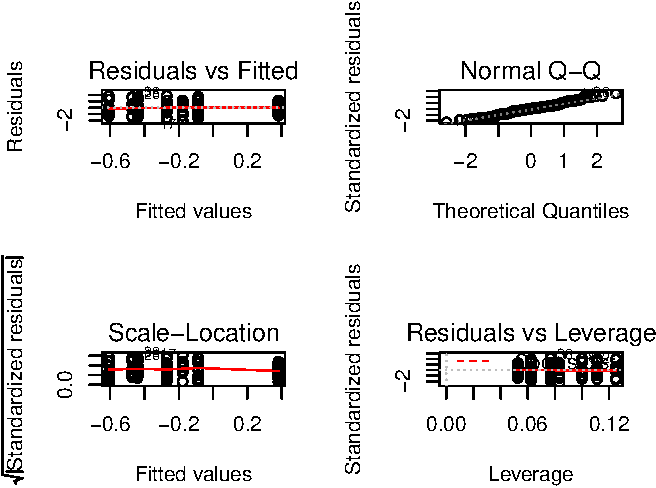
\includegraphics{04_BasicAnalyses_files/figure-beamer/unnamed-chunk-17-1.pdf}

\end{frame}

\begin{frame}[fragile]{Checking Assumptions}

They don't fit great on the slides but trust me that normality looks
good. The assumption of homogeneity of variance looks good as well.

But, if you wanted to test it, you could.

\begin{Shaded}
\begin{Highlighting}[]
\KeywordTok{library}\NormalTok{(car)}
\KeywordTok{leveneTest}\NormalTok{(fit2)}
\end{Highlighting}
\end{Shaded}

\begin{verbatim}
Levene's Test for Homogeneity of Variance (center = median)
      Df F value Pr(>F)
group  7  0.2113 0.9821
      92               
\end{verbatim}

Large p-value here is a good thing: \texttt{emo::ji("smile")}
\footnote{This shows a smiley in `R`, just not on these slides---from the `emo` package on GitHub.}

\end{frame}

\section{Linear Regression}\label{linear-regression}

\begin{frame}{Linear Regression}

\large
Once again, linear regression is essentially the more flexible twin of
ANOVA and
t-tests.\footnote{It mainly only differs from ANOVA in the way it takes a dummy code rather than an effect code of the categorical variables.}

It can:

\begin{enumerate}
\def\labelenumi{\arabic{enumi}.}
\tightlist
\item
  Handle continuous and categorical predictors (i.e., independent
  variables)
\item
  Less stringent assumption of equality of variances
\item
  Is what many other methods are built on (Chapter 5 and 6 will talk
  about some of these)
\end{enumerate}

\end{frame}

\begin{frame}[fragile]{Linear Regression}

We will use \texttt{lm()} (Linear Model) to fit these models.

\small

\begin{Shaded}
\begin{Highlighting}[]
\NormalTok{fit5 =}\StringTok{ }\KeywordTok{lm}\NormalTok{(B }\OperatorTok{~}\StringTok{ }\NormalTok{A, }\DataTypeTok{data =}\NormalTok{ df)}
\KeywordTok{summary}\NormalTok{(fit5)}
\end{Highlighting}
\end{Shaded}

\begin{verbatim}

Call:
lm(formula = B ~ A, data = df)

Residuals:
    Min      1Q  Median      3Q     Max 
-2.2232 -0.5694 -0.0839  0.6275  2.5542 

Coefficients:
            Estimate Std. Error t value Pr(>|t|)
(Intercept)  -0.2291     0.1540  -1.488    0.140
A1            0.1765     0.2039   0.865    0.389

Residual standard error: 1.01 on 98 degrees of freedom
Multiple R-squared:  0.007585,  Adjusted R-squared:  -0.002541 
F-statistic: 0.7491 on 1 and 98 DF,  p-value: 0.3889
\end{verbatim}

\end{frame}

\begin{frame}

\centerline{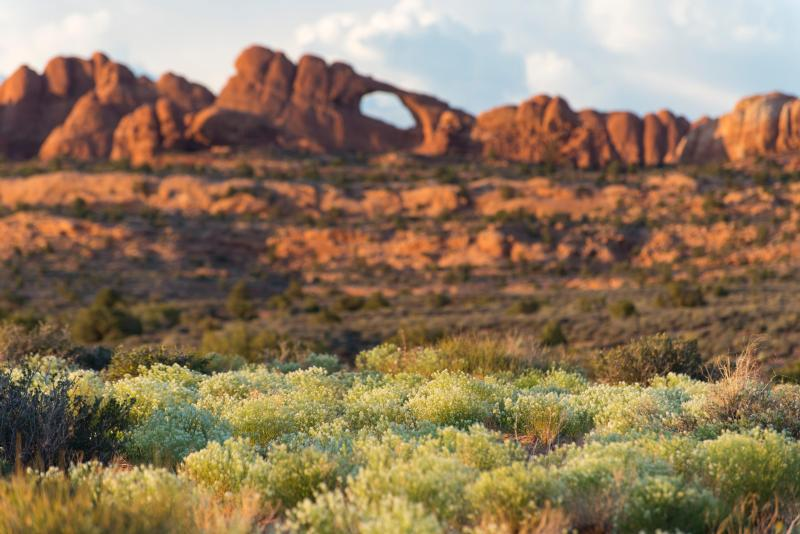
\includegraphics[height=7in]{Figures/grass_landscape_arch.jpg}}

\end{frame}
